
\chapter{Linear PDEs: a structured grid example}
\label{chap:structured}

We start with the Poisson problem on a square---a clich\'e, of course---because it is a straightforward PDE problem on which to learn key parts of \PETSc.  We will build a structured grid using a \pDMDA, then assemble a \pMat in parallel based on this grid, and then solve in parallel using a \pKSP object.  Discretizing the PDE generates a linear system which is only slightly more interesting than the tridiagonal system we solved in Chapter \ref{chap:linearsystem}.

\section{Poisson problem on a square domain}

Let $\mathcal{S}$ be the open unit square $(0,1)\times(0,1)$ with boundary $\partial\mathcal{S}$.  The following is our \emph{Poisson problem} for this Chapter;  see Figure \ref{fig:unitsquare}:
\begin{align}
- \grad^2 u &= f \quad \text{ on } \mathcal{S}, \label{poissonsquare} \\
u &= 0 \quad \text{ on } \partial \mathcal{S}. \label{poissonsquarebcs}
\end{align}
In \eqref{poissonsquare} the \emph{Laplacian} of $u(x,y)$ is
    $$\grad^2 u = \Div(\grad u) = \frac{\partial^2 u}{\partial x^2} + \frac{\partial^2 u}{\partial y^2}.$$

\begin{marginfigure}
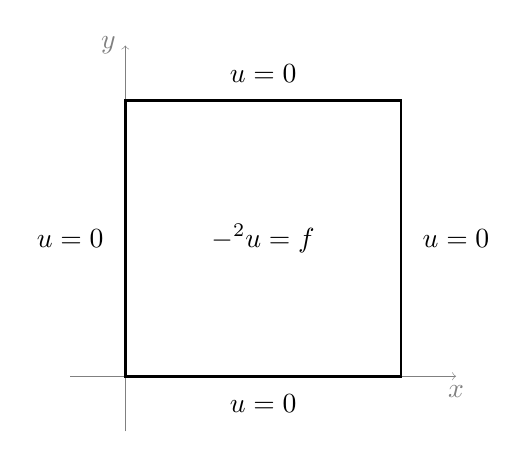
\begin{tikzpicture}[scale=3.5]
  \draw[->,gray,very thin] (-0.2,0.0) -- (1.2,0.0) node[below] {$x$};
  \draw[->,gray,very thin] (0.0,-0.2) -- (0.0,1.2) node[left] {$y$};
  \draw[line width=1.0pt] (0.0,0.0) -- (0.0,1.0) -- (1.0,1.0) -- (1.0,0.0) -- cycle;
  \node at (0.5,0.5) {$- \grad^2 u = f$};
  \node at (0.5,-0.1) {$u = 0$};
  \node at (0.5,1.1) {$u = 0$};
  \node at (-0.2,0.5) {$u = 0$};
  \node at (1.2,0.5) {$u = 0$};
\end{tikzpicture}
\caption{Our first goal is to solve the Poisson equation on the unit square $\mathcal{S}$, with homogeneous Dirichlet boundary conditions.}
\label{fig:unitsquare}
\end{marginfigure}

The next three paragraphs are some standard reminders of the context for equations \eqref{poissonsquare} and \eqref{poissonsquarebcs}.

The Laplacian almost always appears in mathematical models through conservation of $u$, in some sense, along with an assumption that the flux of $u$ is proportional to its gradient \citep{Ockendonetal2003}.  The divergence ``$\Div$'' then arises from the connection between a flux integral over a closed curve or surface and an integral over the interior of that curve or surface, namely the divergence or Gauss-Green theorem \citep[Appendix C]{Evans}.  The \emph{Poisson equation} \eqref{poissonsquare} is subject to \emph{homogeneous Dirichlet} boundary conditions \eqref{poissonsquarebcs} in our problem.  Historically speaking, \eqref{poissonsquare} and \eqref{poissonsquarebcs} form the \emph{Dirichlet problem} if $f=0$ and if the boundary conditions were instead given by some $g$ along $\partial S$.  Nonetheless, we call all instances of the same basic problem ``Poisson.''  We will consider various boundary conditions later (Chapter \ref{chap:unstructured}), always allowing non-zero right-hand sides $f$.  Of course, the problem must have proper types of boundary conditions, either Dirichlet ($u$ known) or Neumann (derivative of $u$ known), or the right combinations, if it is to determine a unique solution.

The Poisson problem may model the electrostatic potential, the equilibrium distribution from certain random walks, or various other other physical phenomena.  For example, in the context of heat conduction in solids Fourier's law says that the heat flux is $\bq = -k \grad u$, where $k$ is the conductivity.  Conservation of heat energy says $c\rho \partial u/\partial t = - \Div\bq + f$ if $f$ describes a heat source within the domain.  The coefficient ``$c\rho$'' parameterizes the ability of the material to hold heat by a gain in temperature \citep{Ockendonetal2003}.  At steady state these facts combine to give Poisson's equation $0 = k \grad^2 u + f$ in the simple case where $k$ is constant.  Holding the temperature fixed at zero along the boundary, i.e.~\eqref{poissonsquarebcs}, completes our version of the problem.

With Dirichlet boundary conditions \eqref{poissonsquarebcs}, the solution to the Poisson problem is unique if it exists.\sidenote{See Theorem 5 in section 2.2 in \citep{Evans} or subsection 5.2.1 of \citep{Ockendonetal2003}.}  On the other hand, holding the heat flux, i.e.~$\grad u$, fixed along the boundary, \emph{Neumann conditions}, is just as common and often more physical.  With only Neumann boundary conditions, however, the Poisson equation $-\grad^2 u = f$ is not a well-posed problem because if $u$ is a solution then $v=u+c$ is also a solution for any constant $c$.  Indeed, without any boundary conditions, there is an infinite-dimensional space of solutions to the Laplace equation $-\grad^2 w = 0$ on $\mathcal{S}$---i.e.~\emph{harmonic functions}---so the Poisson equation is far from well-posed.

In this Chapter we will also require that $f(x,y)$ be continuous and bounded on $\mathcal{S}$, so that we can compute its pointwise values.  With our homogeneous Dirichlet boundary conditions, and this assumption on $f$, standard theory says that $u(x,y)$ exists and is continuous on the closed square $\bar{\mathcal{S}}$ \citep[Theorem 6 in section 5.6]{Evans}.  Thus there is no ambiguity in the boundary condition ``$u=0$ on $\partial \mathcal{S}$.''  Furthermore and we can evaluate pointwise errors if we have an exact solution. 

Because \eqref{poissonsquare} and \eqref{poissonsquarebcs} form a linear problem, finite-dimensional approximations of it are simply linear systems, as solved in the last Chapter.  The approximation in this Chapter comes from applying a \emph{finite difference} (FD) method as a way to generate the linear system.  In the next Chapter we will apply a finite element approach instead.


\section{Building a structured grid}

Our FD method is based on a \emph{structured grid} of $MN$ points on the unit square, as in Figure \ref{fig:unitsquaregrid}, with spacing $h_x=1/(M-1)$ and $h_y=1/(N-1)$ in the two directions.  The grid coordinates are $x_i = i\, h_x$ for $i = 0,1,\dots,M-1$ and $y_j = j\, h_y$ for $j=0,1,\dots,N-1$.  The construction of such a 2D grid, and distributing it across processors, are our first new ideas from \PETSc beyond the basics in Chapters \ref{chap:getstarted} and \ref{chap:linearsystem}.

\begin{marginfigure}
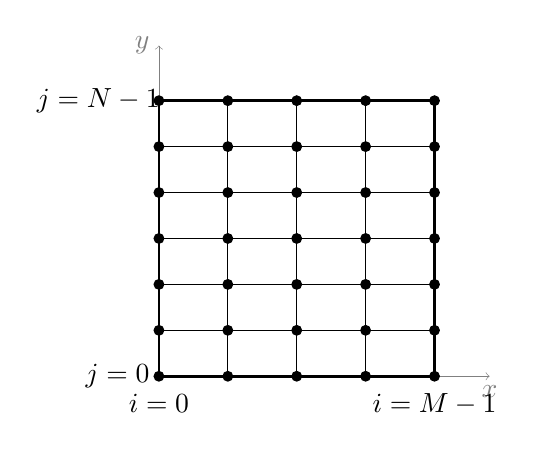
\begin{tikzpicture}[scale=3.5]
  \draw[->,gray,very thin] (0.0,0.0) -- (1.2,0.0) node[below] {$x$};
  \draw[->,gray,very thin] (0.0,0.0) -- (0.0,1.2) node[left] {$y$};
  \draw[line width=1.0pt] (0.0,0.0) -- (0.0,1.0) -- (1.0,1.0) -- (1.0,0.0) -- cycle;
  \node at (0.0,-0.1) {$i=0$};
  \node at (1.0,-0.1) {$i=M-1$};
  \node at (-0.15,0.0) {$j=0$};
  \node at (-0.22,1.0) {$j=N-1$};
  \pgfmathsetmacro\fourth{1.0/4.0}
  \pgfmathsetmacro\sixth{1.0/6.0}
  \draw[xstep=\fourth,ystep=\sixth,black,thin] (0.0,0.0) grid (1.0,1.0);
  \foreach \x in {0,...,4} {
    \foreach \y in {0,...,6} {
        \filldraw (\x * \fourth,\y * \sixth) circle (0.5pt);
    }
  }
\end{tikzpicture}
\caption{A grid on the unit square $\mathcal{S}$, with $M=5$ and $N=7$.}
\label{fig:unitsquaregrid}
\end{marginfigure}

Consider the lines of code in Figure \ref{code:dmdacreatetwod}, an extract from \texttt{poisson.c} later in this Chapter.  These lines create a \PETSc \pDM object for a grid like Figure \ref{fig:unitsquaregrid}.  A \pDM is an abstract type for describing the topology (connectedness) and geometry of a grid, \emph{and} the way it is distributed across \MPI processes, \emph{and} the way each process can access data from its neighboring processes.  The specific case in Figure \ref{code:dmdacreatetwod} creates a ``\pDMDA'', the subclass of \pDM s which are structured grids.  (Note ``\pDM'' might stand for ``distributed mesh,'' and ``\texttt{DA}'' for ``distributed array''.)

\cinputraw{dmdacreate2d.frag}{extract from c/ch3/poisson.c}{An example of creating a 2D \pDMDA.  See Figures \ref{code:poissoncreate} and \ref{code:poissonsolve} for the rest of this code.}{}{//START}{//STOP}{code:dmdacreatetwod}

\begin{marginfigure}
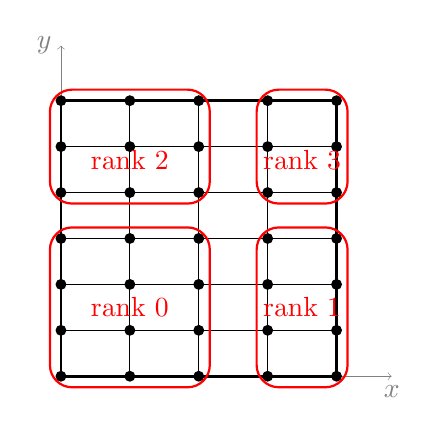
\begin{tikzpicture}[scale=3.5]
  \draw[->,gray,very thin] (0.0,0.0) -- (1.2,0.0) node[below] {$x$};
  \draw[->,gray,very thin] (0.0,0.0) -- (0.0,1.2) node[left] {$y$};
  \draw[line width=1.0pt] (0.0,0.0) -- (0.0,1.0) -- (1.0,1.0) -- (1.0,0.0) -- cycle;
  \pgfmathsetmacro\fourth{1.0/4.0}
  \pgfmathsetmacro\sixth{1.0/6.0}
  \draw[xstep=\fourth,ystep=\sixth,black,thin] (0.0,0.0) grid (1.0,1.0);
  \foreach \x in {0,...,4} {
    \foreach \y in {0,...,6} {
        \filldraw (\x * \fourth,\y * \sixth) circle (0.5pt);
    }
  }
  \pgfmathsetmacro\dd{0.04}
  \pgfmathsetmacro\od{1.04}
  \pgfmathsetmacro\xap{2*\fourth + 0.04}
  \pgfmathsetmacro\xbm{3*\fourth - 0.04}
  \pgfmathsetmacro\yap{3*\sixth + 0.04}
  \pgfmathsetmacro\ybm{4*\sixth - 0.04}
  \pgfmathsetmacro\xamid{1*\fourth}
  \pgfmathsetmacro\xbmid{3.5*\fourth}
  \pgfmathsetmacro\yamid{1.5*\sixth}
  \pgfmathsetmacro\ybmid{4.7*\sixth}
  \draw[thick,rounded corners=8pt,color=red]
    (-\dd,-\dd) -- (-\dd,\yap) -- (\xap,\yap) -- (\xap,-\dd) -- cycle;
  \node[color=red] at (\xamid,\yamid) {rank $0$};
  \draw[thick,rounded corners=8pt,color=red]
    (\xbm,-\dd) -- (\od,-\dd) -- (\od,\yap) -- (\xbm,\yap) -- cycle;
  \node[color=red] at (\xbmid,\yamid) {rank $1$};
  \draw[thick,rounded corners=8pt,color=red]
    (-\dd,\ybm) -- (\xap,\ybm) -- (\xap,\od) -- (-\dd,\od) -- cycle;
  \node[color=red] at (\xamid,\ybmid) {rank $2$};
  \draw[thick,rounded corners=8pt,color=red]
    (\xbm,\ybm) -- (\od,\ybm) -- (\od,\od) -- (\xbm,\od) -- cycle;
  \node[color=red] at (\xbmid,\ybmid) {rank $3$};
\end{tikzpicture}
\caption{The same grid as in Figure \ref{fig:unitsquaregrid}, distributed across four \MPI processes (i.e.~with \texttt{rank} $\in \{0,1,2,3\}$) automatically by \texttt{DMDACreate2d()}.}
\label{fig:unitsquaregridparallel}
\end{marginfigure}

If we do
\begin{cline}
$ cd c/ch3/
$ make poisson
$ ./poisson -da_grid_x 5 -da_grid_y 7
\end{cline}
%$
then the structured grid shown in Figure \ref{fig:unitsquaregrid} is created.  In this case all points of the grid are ``owned'' by a single MPI process.  However, if we run with multiple \MPI processes by
\begin{cline}
$ mpiexec -n K ./poisson -da_grid_x M -da_grid_y N
\end{cline}
%$
then \PETSc does the best it can to balance the load of \texttt{MN} grid points among \texttt{K} processes, with the restriction that each \MPI process owns a rectangular subgrid.  For example,
\begin{cline}
$ mpiexec -n 4 ./poisson -da_grid_x 5 -da_grid_y 7
\end{cline}
%$
distributes the grid as shown in Figure \ref{fig:unitsquaregridparallel} will be created.  Neither \texttt{M}$=5$ nor \texttt{N}$=7$ is divisible by two, but \PETSc distributes the four ranks across the \texttt{MN}$=35$ nodes (grid points) relatively uniformly: the rank $0$ process owns 12 grid points and rank $3$ owns 6, while the other ranks are in between.  In this case the load is only balanced to within a factor of two, but larger grids can be better load-balanced.

\begin{marginfigure}
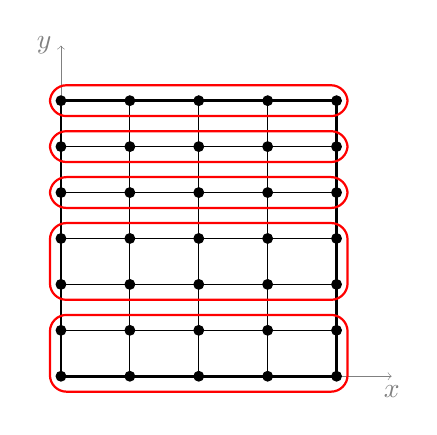
\begin{tikzpicture}[scale=3.5]
  \draw[->,gray,very thin] (0.0,0.0) -- (1.2,0.0) node[below] {$x$};
  \draw[->,gray,very thin] (0.0,0.0) -- (0.0,1.2) node[left] {$y$};
  \draw[line width=1.0pt] (0.0,0.0) -- (0.0,1.0) -- (1.0,1.0) -- (1.0,0.0) -- cycle;
  \pgfmathsetmacro\fourth{1.0/4.0}
  \pgfmathsetmacro\sixth{1.0/6.0}
  \draw[xstep=\fourth,ystep=\sixth,black,thin] (0.0,0.0) grid (1.0,1.0);
  \foreach \x in {0,...,4} {
    \foreach \y in {0,...,6} {
        \filldraw (\x * \fourth,\y * \sixth) circle (0.5pt);
    }
  }
  \pgfmathsetmacro\dd{0.04}
  \pgfmathsetmacro\od{1.04}
  \foreach \y in {0,2} {
    \pgfmathsetmacro\yup{\y * \sixth - 1.4 * \dd}  % less than 1.7 generates flaw?
    \pgfmathsetmacro\ydn{(\y + 1) * \sixth + 1.4 * \dd}
    \draw[thick,rounded corners=6pt,color=red]
      (-\dd,\ydn) -- (\od,\ydn) -- (\od,\yup) -- (-\dd,\yup) -- cycle;
  }
  \foreach \y in {4,5,6} {
    \pgfmathsetmacro\yup{\y * \sixth - 1.4 * \dd}  % less than 1.7 generates flaw?
    \pgfmathsetmacro\ydn{\y * \sixth + 1.4 * \dd}
    \draw[thick,rounded corners=6pt,color=red]
      (-\dd,\ydn) -- (\od,\ydn) -- (\od,\yup) -- (-\dd,\yup) -- cycle;
  }
\end{tikzpicture}
\caption{Processor domains are far from square if the number of \MPI processes is prime.}
\label{fig:unitsquaregridprime}
\end{marginfigure}

The observant reader has already noted that if the total number of processes \texttt{K}, in ``\texttt{mpiexec -n K},'' is prime then we get not-at-all-square processor domains.  For instance, the ``bad'' result from running
\begin{cline}
$ mpiexec -n 5 ./poisson -da_grid_x 5 -da_grid_y 7
\end{cline}
%$
is shown in Figure \ref{fig:unitsquaregridprime}.  Each process' portion of the grid has large perimeter-to-area ratio.  Thus communication between processes will be large compared to the computation on each process.

\begin{marginfigure}
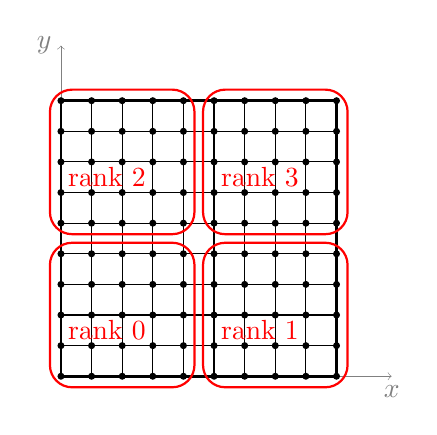
\begin{tikzpicture}[scale=3.5]
  \draw[->,gray,very thin] (0.0,0.0) -- (1.2,0.0) node[below] {$x$};
  \draw[->,gray,very thin] (0.0,0.0) -- (0.0,1.2) node[left] {$y$};
  \draw[line width=1.0pt] (0.0,0.0) -- (0.0,1.0) -- (1.0,1.0) -- (1.0,0.0) -- cycle;
  \pgfmathsetmacro\ninth{1.0/9.0}
  \draw[xstep=\ninth,ystep=\ninth,black,thin] (0.0,0.0) grid (1.0,1.0);
  \foreach \x in {0,...,9} {
    \foreach \y in {0,...,9} {
        \filldraw (\x * \ninth,\y * \ninth) circle (0.3pt);
    }
  }
  \pgfmathsetmacro\dd{0.04}
  \pgfmathsetmacro\od{1.04}
  \pgfmathsetmacro\ap{4*\ninth + 0.04}
  \pgfmathsetmacro\bm{5*\ninth - 0.04}
  \pgfmathsetmacro\amid{1.5*\ninth}
  \pgfmathsetmacro\bmid{6.5*\ninth}
  \draw[thick,rounded corners=8pt,color=red]
    (-\dd,-\dd) -- (-\dd,\ap) -- (\ap,\ap) -- (\ap,-\dd) -- cycle;
  \node[color=red] at (\amid,\amid) {rank $0$};
  \draw[thick,rounded corners=8pt,color=red]
    (\bm,-\dd) -- (\od,-\dd) -- (\od,\ap) -- (\bm,\ap) -- cycle;
  \node[color=red] at (\bmid,\amid) {rank $1$};
  \draw[thick,rounded corners=8pt,color=red]
    (-\dd,\bm) -- (\ap,\bm) -- (\ap,\od) -- (-\dd,\od) -- cycle;
  \node[color=red] at (\amid,\bmid) {rank $2$};
  \draw[thick,rounded corners=8pt,color=red]
    (\bm,\bm) -- (\od,\bm) -- (\od,\od) -- (\bm,\od) -- cycle;
  \node[color=red] at (\bmid,\bmid) {rank $3$};
\end{tikzpicture}
\caption{A well-balanced, compact-domain distribution of a $M=10$ by $N=10$ grid across four \MPI processes, created by \texttt{DMDACreate2d()}.}
\label{fig:unitsquaregrideight}
\end{marginfigure}

Though these defaults can be overridden by runtime options \texttt{-da\_grid\_x} and \texttt{-da\_grid\_y}, the fifth and sixth arguments ``\texttt{-9}'' of \texttt{DMDACreate2d()} in Figure \ref{code:dmdacreatetwod} are used to set default dimensions $M=9$ and $N=9$.  Thus
\begin{cline}
$ mpiexec -n 4 ./poisson
\end{cline}
%$
distributes the default $9\times 9$ grid in a well-balanced manner among four processes.  Figure \ref{fig:unitsquaregrideight} shows the perfectly-balanced result of
\begin{cline}
$ mpiexec -n 4 ./poisson -da_grid_x 10 -da_grid_y 10
\end{cline}
%$
with each rank owning a square subgrid of 25 nodes.

To explain the other options to \texttt{DMDACreate2d()} we quote the \PETSc manual pages description:

\begin{code}
DMDACreate2d(MPI_Comm comm, DMBoundaryType bx, DMBoundaryType by,
  DMDAStencilType stype, PetscInt M, PetscInt N, PetscInt m, PetscInt n,
  PetscInt dof, PetscInt s, const PetscInt lx[], const PetscInt ly[],
  DM *da)
\end{code}
where
\small
\begin{itemize}[align=left]
\item[\texttt{comm}]   MPI communicator \\
\item[\texttt{bx,by}]  type of ghost nodes the array have; use one of \texttt{DM\_BOUNDARY\_NONE, DM\_BOUNDARY\_GHOSTED, DM\_BOUNDARY\_PERIODIC} \\
\item[\texttt{stype}] stencil type; use either \texttt{DMDA\_STENCIL\_BOX} or \texttt{DMDA\_STENCIL\_STAR} \\
\item[\texttt{M,N}]	   global dimension in each direction of the array; use \texttt{-M} and or \texttt{-N} to indicate that it may be set to a different value from the command line with \texttt{-da\_grid\_x <M> -da\_grid\_y <N>} \\
\item[\texttt{m,n}]   corresponding number of processors in each dimension (or \texttt{PETSC\_DECIDE} to have calculated) \\
\item[\texttt{dof}]     number of degrees of freedom per node \\
\item[\texttt{s}]       stencil width \\
\item[\texttt{lx,ly}]  arrays containing the number of nodes in each cell along the x and y coordinates, or \texttt{NULL}; if non-null, these must be of length as m and n, and the corresponding m and n cannot be \texttt{PETSC\_DECIDE}; the sum of the \texttt{lx[]} entries must be M, and the sum of the \texttt{ly[]} entries must be N \\
\item[\texttt{da}]      output: the resulting distributed array object 
\end{itemize}
\normalsize

In Figure \ref{code:dmdacreatetwod}, the second and third arguments are \texttt{DM\_BOUNDARY\_NONE} because our Dirichlet boundary conditions do not need communication to the next process' domain, nor periodic wrapping.  In the fourth argument we use \texttt{DMDA\_STENCIL\_STAR} because only cardinal neighbors of a grid point are used when forming the matrix.\sidenote{Figure \ref{fig:unitsquaregridstencil} shows the ``stencil'' of our FD method.}  The two \texttt{PETSC\_DECIDE} arguments which follow tell \PETSc to distribute the grid over processes according to the size of (number of processes in) the \MPI communicator, and using \PETSc internal logic as illustrated above.  The next two arguments, in the ninth and tenth positions, say that our PDE is scalar (\texttt{dof}$=1$) and that the FD method only needs one neighbor in each direction (\texttt{s}$=1$).  The next two arguments after that are \texttt{NULL} because we are \emph{not} telling \PETSc any details about how to distribute processes over the grid; it \texttt{DECIDE}s for itself.  Finally, the \pDMDA object is created as an output (i.e.~pass-by-reference).

The call to \texttt{DMDASetUniformCoordinates()} in Figure \ref{code:dmdacreatetwod} sets the domain to be $[0,1]\times[0,1]$ in the sense that the \pDM object knows the spacing and locations of the grid points.  The last two arguments are ignored in this case; they would set limits on the third dimension if \texttt{da} were created with \texttt{DMDACreate3d()}.

\medskip
\begin{figure}
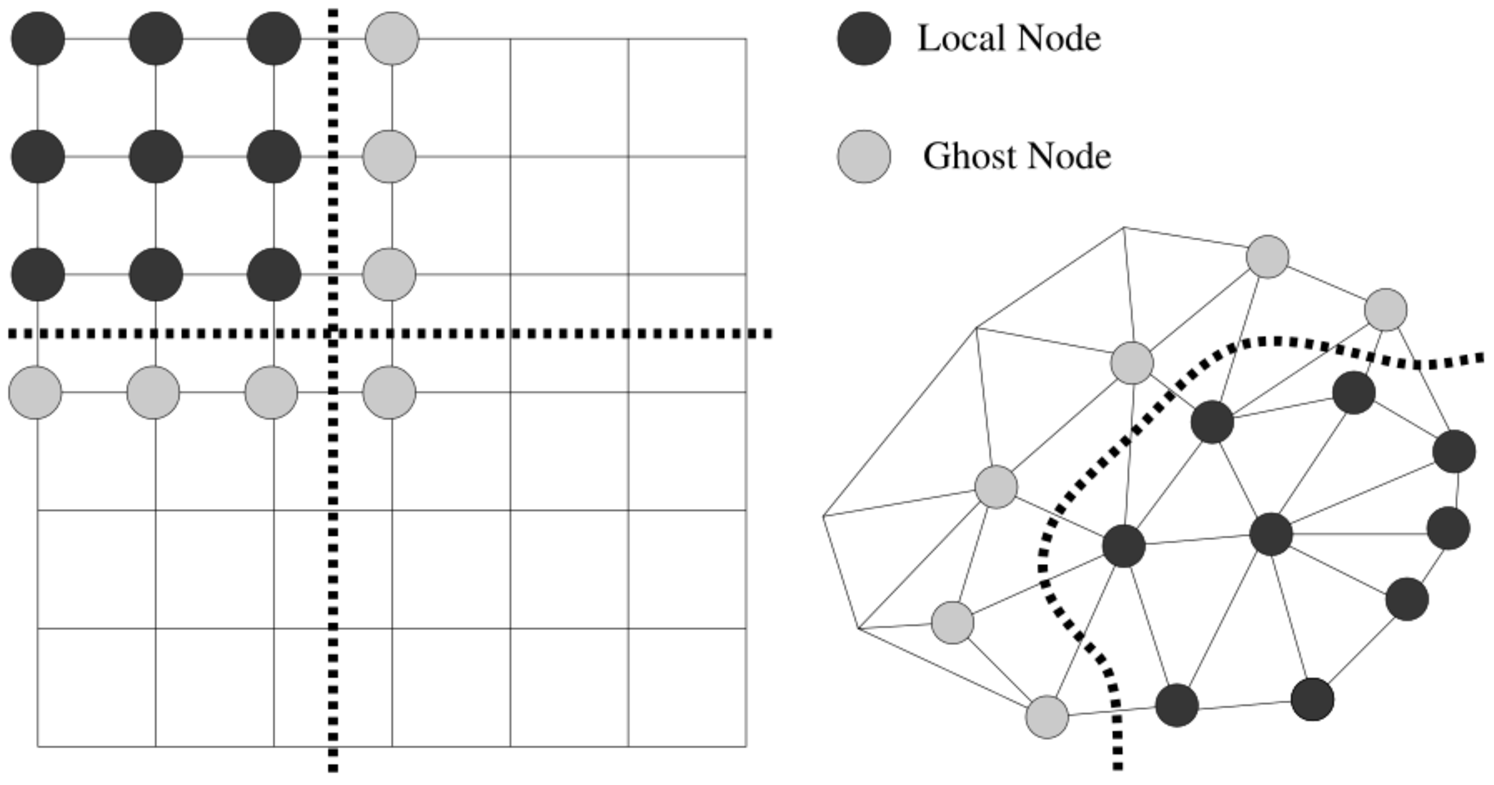
\includegraphics[width=\textwidth]{petscghostvalues}
\caption{\PETSc's parallel decomposition of structured (left) and unstructured (right) grids, showing owned (``local'') and accessible (``ghost'') nodes for one process.}
\label{fig:petscghostvalues}
\end{figure}

The standard \PETSc view of what \pDM s ``look like'' is in Figure \ref{fig:petscghostvalues}.  The code in Figure \ref{code:dmdacreatetwod} generates something like the left figure, namely a structured-grid \pDM, except that the one shown in Figure \ref{fig:petscghostvalues} has \texttt{DMDA\_STENCIL\_BOX} stencil type, unlike ours.  On the right is an unstructured grid, of the type created in Chapter \ref{chap:unstructured} for the finite element method.  In both cases the Figure shows the nodes owned by a given process (red ``local'' nodes) and those other nodes that are accessible by the local process (blue ``ghost'' nodes).


\section{Finite difference method}

Recall we were trying to approximate PDE problem \eqref{poissonsquare} and \eqref{poissonsquarebcs}, not just build a grid.  The following FD method leads to the next step, creating and assembling a \pMat, and some \pVecs, for the linear system corresponding to the PDE.

By a well-known Taylor's theorem argument \citep{MortonMayers}, if $F(x)$ is sufficiently smooth then
\begin{equation}
   F''(x) = \frac{F(x+h) - 2 F(x) + F(x-h)}{h^2} + O(h^2)  \label{secondderivativeFD}
\end{equation}
as $h$ goes to zero.  This formula, applied to partial derivatives, will approximate the Laplacian in equation \eqref{poissonsquare}.  In fact, if $U_{i,j}$ is the gridded approximation to the value $u(x_i,y_j)$ of the exact solution $u(x,y)$ at a grid point,\sidenote{This is an important phrase!  We compute values $U_{i,j}$ from the finite difference equations.  We generally \emph{do not know} the values $u(x_i,y_j)$.  We want the former to be close to the latter.} and if $f_{i,j} = f(x_i,y_j)$ then from \eqref{secondderivativeFD} we have this FD approximation to equation \eqref{poissonsquare}:
\begin{equation}
- \frac{U_{i+1,j} - 2 U_{i,j} + U_{i-1,j}}{h_x^2} - \frac{U_{i,j+1} - 2 U_{i,j} + U_{i,j-1}}{h_y^2} = f_{i,j}. \label{poissonsquareFDearly}
\end{equation}
Equation \eqref{poissonsquareFDearly} applies at all interior points where $1 \le i \le M-2$ and $1 \le j \le N-2$.  The boundary conditions \eqref{poissonsquarebcs} become
\begin{equation}
U_{0,j} = 0, \quad U_{M-1,j} = 0, \quad U_{i,0} = 0, \quad U_{i,N-1} = 0, \label{poissonsquareFDbcs}
\end{equation}
for all $i,j$.

At grid location $(x_i,y_j)$, equation \eqref{poissonsquareFDearly} relates the unknown $U_{i,j}$ to its four cardinal neighbors $U_{i+1,j}$, $U_{i-1,j}$, $U_{i,j+1}$, and $U_{i,j-1}$.  This pattern is a \emph{stencil}, in particular a ``star'' stencil, as shown in Figure \ref{fig:unitsquaregridstencil}.  By contrast, a ``box'' stencil would additionally involve the four diagonal neighbors.  In 2D, a star stencil relates five unknowns, while a box stencil relates nine unknowns.

\begin{marginfigure}
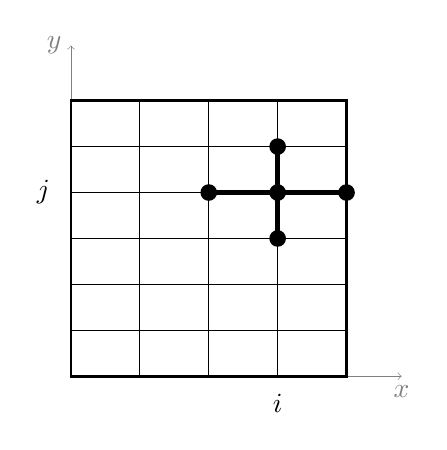
\begin{tikzpicture}[scale=3.5]
  \draw[->,gray,very thin] (0.0,0.0) -- (1.2,0.0) node[below] {$x$};
  \draw[->,gray,very thin] (0.0,0.0) -- (0.0,1.2) node[left] {$y$};
  \draw[line width=1.0pt] (0.0,0.0) -- (0.0,1.0) -- (1.0,1.0) -- (1.0,0.0) -- cycle;
  \node at (0.75,-0.1) {$i$};
  \node at (-0.1,0.666667) {$j$};
  \filldraw (0.50,0.666667) circle (0.8pt);
  \filldraw (0.75,0.666667) circle (0.8pt);
  \filldraw (1.00,0.666667) circle (0.8pt);
  \filldraw (0.75,0.5) circle (0.8pt);
  \filldraw (0.75,0.833333) circle (0.8pt);
  \draw[line width=2.0pt] (0.50,0.666667) -- (1.00,0.666667);
  \draw[line width=2.0pt] (0.75,0.5)  -- (0.75,0.833333);
  \draw[xstep=0.25,ystep=0.166667,black,thin] (0.0,0.0) grid (1.0,1.0);
\end{tikzpicture}
\caption{This ``star'' stencil simply illustrates the adjacency pattern in FD scheme \eqref{poissonsquareFDearly}.}
\label{fig:unitsquaregridstencil}
\end{marginfigure}

We will treat all values $U_{i,j}$ as unknowns, whether on the boundary or in the interior, so we have $L=MN$ unknowns.  Equations \eqref{poissonsquareFDearly} and \eqref{poissonsquareFDbcs} form a linear system of $L$ equations,
\begin{equation}
A \bu = \bb, \label{poissonlinearsystem}
\end{equation}
where $A$ is a $L\times L$ matrix and $\bu,\bb$ are $L\times 1$ column vectors.

However, to show entries of $A$ and $\bb$ in linear system \eqref{poissonlinearsystem} we must globally-order the unknowns.  Such an ordering is implemented inside a \PETSc \pDMDA, and indeed our code (\texttt{poisson.c} below) will use only the grid-wise coordinates $(i,j)$.\sidenote{The ability to assemble \pMats and \pVecs with $(i,j)$-type indexing is one reason structured-grid codes using \pDMDA can be quite short.}  Here we expose the ordering only for the purpose of displaying the system in matrix-vector form.

The ordering used in a one-process (serial) run by a 2D \pDMDA is shown in Figure \ref{fig:unitsquaregridordering}.  On an $M$ by $N$ grid one could write it as
\begin{equation}
    U_k = U_{i,j} \quad \text{ where } \quad k = j\,M + i \label{orderingfd}
\end{equation}
for $i=0,1,\dots,M-1$ and $j=0,1,\dots,N-1$, so $k=0,1,\dots,MN-1$.  Of course we let \PETSc do such index transformations inside the \pDMDA implementation.

\begin{marginfigure}
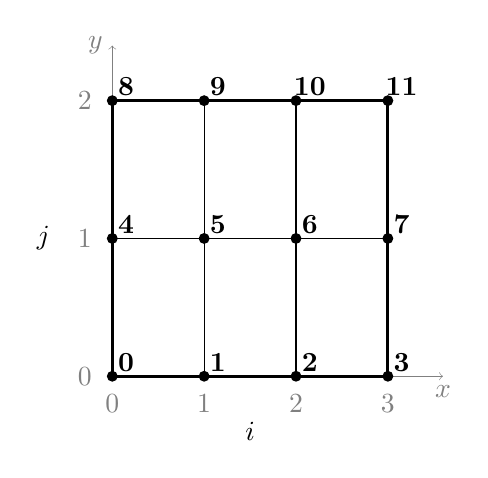
\begin{tikzpicture}[scale=3.5]
  \draw[->,gray,very thin] (0.0,0.0) -- (1.2,0.0) node[below] {$x$};
  \draw[->,gray,very thin] (0.0,0.0) -- (0.0,1.2) node[left] {$y$};
  \draw[line width=1.0pt] (0.0,0.0) -- (0.0,1.0) -- (1.0,1.0) -- (1.0,0.0) -- cycle;
  \pgfmathsetmacro\third{1.0/3.0}
  \pgfmathsetmacro\half{1.0/2.0}
  \node[gray] at (0.0,-0.1) {$0$};
  \node[gray] at (\third,-0.1) {$1$};
  \node at (\half,-0.2) {$i$};
  \node[gray] at (2*\third,-0.1) {$2$};
  \node[gray] at (1.0,-0.1) {$3$};
  \node[gray] at (-0.1,0.0) {$0$};
  \node[gray] at (-0.1,0.5) {$1$};
  \node at (-0.25,0.5) {$j$};
  \node[gray] at (-0.1,1.0) {$2$};
  \draw[xstep=\third,ystep=\half,black,thin] (0.0,0.0) grid (1.0,1.0);
  \pgfmathsetmacro\dd{0.05}
  \foreach \y in {0,1,2}
    \foreach \x in {0,1,2,3} {
      \pgfmathsetmacro\k{4*\y+\x}
      \draw (\x*\third+\dd,\y*\half+\dd) node{$\mathbf{\pgfmathprintnumber[fixed]{\k}}$};
      \filldraw (\x * \third,\y * \half) circle (0.5pt);
    }
\end{tikzpicture}
\caption{Ordering of unknowns \eqref{orderingfd} on a $M=4$ and $N=3$ grid.  Index $k$ from \eqref{orderingfd} is shown in \textbf{bold}.}
\label{fig:unitsquaregridordering}
\end{marginfigure}

\medskip\noindent\hrulefill
\begin{example} In the $M=4$ and $N=3$ case (Figure \ref{fig:unitsquaregridordering}) we have grid spacing $h_x=1/3$ and $h_y=1/2$.  Only the $k=5$ and $k=6$ equations are not boundary conditions \eqref{poissonsquareFDbcs}.  The linear system \eqref{poissonlinearsystem} is
\setcounter{MaxMatrixCols}{20}
\begin{equation*}
\begin{bmatrix}
1 &  &  &  &  &  &  &  &  &  &  &  \\
  & 1&  &  &  &  &  &  &  &  &  &  \\
  &  & 1&  &  &  &  &  &  &  &  &  \\
  &  &  & 1&  &  &  &  &  &  &  &  \\
  &  &  &  & 1&  &  &  &  &  &  &  \\
  & c&  &  & b& a& b&  &  & c&  &  \\
  &  & c&  &  & b& a& b&  &  & c&  \\
  &  &  &  &  &  &  & 1&  &  &  &  \\
  &  &  &  &  &  &  &  & 1&  &  &  \\
  &  &  &  &  &  &  &  &  & 1&  &  \\
  &  &  &  &  &  &  &  &  &  & 1&  \\
  &  &  &  &  &  &  &  &  &  &  & 1
\end{bmatrix}
\begin{bmatrix}
U_{0,0} \\
U_{1,0} \\
U_{2,0} \\
U_{3,0} \\
U_{0,1} \\
U_{1,1} \\
U_{2,1} \\
U_{3,1} \\
U_{0,2} \\
U_{1,2} \\
U_{2,2} \\
U_{3,2}
\end{bmatrix}
=
\begin{bmatrix}
0 \\
0 \\
0 \\
0 \\
0 \\
f_{1,1} \\
f_{2,1} \\
0 \\
0 \\
0 \\
0 \\
0
\end{bmatrix}
\end{equation*}
where $a = 2/h_x^2 + 2/h_y^2 = 26$, $b = - 1/h_x^2 = -9$ and $c = - 1/h_y^2 = -4$.

The matrix $A$ is not symmetric.  Furthermore it is not well-scaled, for such a small example, because the 2-norm condition number is $\kappa(A) = \|A\|_2 \|A^{-1}\|_2 = 43.16$.
\end{example}
\noindent\hrulefill

\medskip
Before assembling the system by writing \PETSc code, there are two nontrivial observations about it.  These observations lead to an equivalent linear system that is easier to solve both in the sense that we have more options for solving the system,\sidenote{More \pKSP and \pPC choices and more choices that converge.} and in the sense that the numerical solution is more accurate because the condition number is smaller.\sidenote{Recall idea i) on page \pageref{limittoaccuracy}.}

First, equations \eqref{poissonsquareFDearly} have very different ``scaling'' from equations \eqref{poissonsquareFDbcs}.  For example, if $M=N=1001$, so that $h_x=h_y=0.001$, then the coefficient of $U_{i,j}$ in \eqref{poissonsquareFDearly} is $4/(.001)^2 = 4 \times 10^6$, while the coefficients from \eqref{poissonsquareFDbcs} are equal to 1.  To make the equations better scaled, we multiply \eqref{poissonsquareFDearly} by the grid cell area $h_x h_y$ to get
\begin{equation}
2 (a + b) U_{i,j} - a \left(U_{i+1,j} + U_{i-1,j}\right) - b \left(U_{i,j+1} + U_{i,j-1}\right) = h_x h_y f_{i,j} \label{poissonsquareFD}
\end{equation}
where $a=h_y/h_x$ and $b=h_x/h_y$.  Using \eqref{poissonsquareFD}, all the equations in the system will have coefficients of comparable size, unless the cell aspect ratio $h_y/h_x$ is very large or small.  If $h_x=h_y$ then diagonal entries are $4$ and off-diagonal entries are $-1$ as in Figure \ref{fig:equalstarstencil}.

\begin{marginfigure}
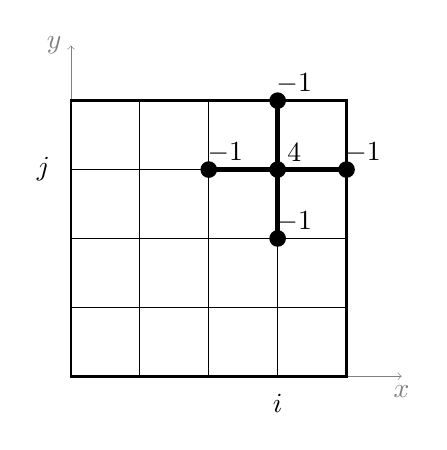
\begin{tikzpicture}[scale=3.5]
  \draw[->,gray,very thin] (0.0,0.0) -- (1.2,0.0) node[below] {$x$};
  \draw[->,gray,very thin] (0.0,0.0) -- (0.0,1.2) node[left] {$y$};
  \draw[line width=1.0pt] (0.0,0.0) -- (0.0,1.0) -- (1.0,1.0) -- (1.0,0.0) -- cycle;
  \node at (0.75,-0.1) {$i$};
  \node at (-0.1,0.75) {$j$};
  \filldraw (0.50,0.75) circle (0.8pt);
  \filldraw (0.75,0.75) circle (0.8pt);
  \filldraw (1.00,0.75) circle (0.8pt);
  \filldraw (0.75,0.5) circle (0.8pt);
  \filldraw (0.75,1.0) circle (0.8pt);
  \pgfmathsetmacro\dd{0.06}
  \draw (0.75+\dd,0.75+\dd) node{$4$};
  \draw (0.5+\dd,0.75+\dd)  node{$-1$};
  \draw (0.75+\dd,0.5+\dd)  node{$-1$};
  \draw (1.0+\dd,0.75+\dd)  node{$-1$};
  \draw (0.75+\dd,1.0+\dd)  node{$-1$};
  \draw[line width=2.0pt] (0.50,0.75) -- (1.00,0.75);
  \draw[line width=2.0pt] (0.75,0.5)  -- (0.75,1.00);
  \draw[xstep=0.25,ystep=0.25,black,thin] (0.0,0.0) grid (1.0,1.0);
\end{tikzpicture}
\caption{For a grid with $h_x=h_y$, the coefficients on the left side of \eqref{poissonsquareFD} are the well-known ``$4$'' and ``$-1$'' for the stencil of the Laplacian.}
\label{fig:equalstarstencil}
\end{marginfigure}

Our second observation is that the FD equations can be re-interpreted to give a \emph{symmetric} matrix $A$.  For example, at a grid point adjacent to the left-hand boundary of the square, the $i=1$ case of \eqref{poissonsquareFD}, the boundary location value $U_{0,j}$ appears in the equation.  The matrix in the linear system will be symmetric if we systematically ``move'' such values to the right-hand side vector $\bb$, as the value $U_{0,j}$ is known.  That is, we force off-diagonal entries $A$ to be zero in columns corresponding to known boundary values.  With these two modifications we can redo the last example.

\medskip\noindent\hrulefill
\begin{example} \label{exampleredo} For the same $M=4$ and $N=3$ case shown in Figure \ref{fig:unitsquaregridordering}, equations \eqref{poissonsquareFDbcs} and \eqref{poissonsquareFD} yield the linear system
\begin{equation*}
\begin{bmatrix}
1 &  &  &  &  &  &  &  &  &  &  &  \\
  & 1&  &  &  &  &  &  &  &  &  &  \\
  &  & 1&  &  &  &  &  &  &  &  &  \\
  &  &  & 1&  &  &  &  &  &  &  &  \\
  &  &  &  & 1&  &  &  &  &  &  &  \\
  &  &  &  &  & \alpha& \beta&  &  &  &  &  \\
  &  &  &  &  & \beta& \alpha&  &  &  &  &  \\
  &  &  &  &  &  &  & 1&  &  &  &  \\
  &  &  &  &  &  &  &  & 1&  &  &  \\
  &  &  &  &  &  &  &  &  & 1&  &  \\
  &  &  &  &  &  &  &  &  &  & 1&  \\
  &  &  &  &  &  &  &  &  &  &  & 1
\end{bmatrix}
\begin{bmatrix}
U_{0,0} \\
U_{1,0} \\
U_{2,0} \\
U_{3,0} \\
U_{0,1} \\
U_{1,1} \\
U_{2,1} \\
U_{3,1} \\
U_{0,2} \\
U_{1,2} \\
U_{2,2} \\
U_{3,2}
\end{bmatrix}
=
\begin{bmatrix}
0 \\
0 \\
0 \\
0 \\
0 \\
(1/6) f_{1,1} \\
(1/6) f_{2,1} \\
0 \\
0 \\
0 \\
0 \\
0
\end{bmatrix}
\end{equation*}
where $\alpha = 2 (h_y/h_x) + 2 (h_x/h_y) = 13/3$ and $\beta = - h_y/h_x = - 3/2$.  The matrix is symmetric, positive definite, and better-scaled than before with $\kappa(A)=5.83$.
\end{example}
\noindent\hrulefill

By converting the earlier system to a symmetric matrix $A$ we open up a larger range of linear algebra methods for solving the system efficiently.  We can now use conjugate gradients as the \pKSP (\texttt{-ksp\_type cg}), plus Cholesky preconditioners (\texttt{-pc\_type cholesky} or \texttt{-pc\_type icc}).


\section{Code for matrix assembly}

We now show in Figure \ref{code:structuredpoisson} the code that assembles ``$A$'' in linear system \eqref{poissonlinearsystem} using \eqref{poissonsquareFD}.  For clarity and code reuse we have isolated this method in a separate file.  Arguments to \texttt{formdirichletlaplacian()} are simply the \pDM, the value to put on the diagonal for Dirichlet boundary conditions,\sidenote{This changes in a time-dependent problem which reuses the code} and the returned (i.e.~modified) \pMat \texttt{A}.

\cinputpart{structuredpoisson.c}{c/ch3/}{Fill matrix entries using \texttt{MatSetValuesStencil}.  (From now on we strip ``\texttt{ierr=}'' and ``\texttt{CHKERRQ(ierr)}'' from the displayed code, but it is still present in the source.)}{I}{//CREATEMATRIX}{//ENDCREATEMATRIX}{code:structuredpoisson}

The ``\texttt{DMDALocalInfo info}'' object needs special description.  It is a C structure which stores both global grid size and the extent of the locally-owned subgrid, as shown in Figure \ref{fig:localpartofgrid}.  The global size is in members \texttt{info.mx,info.my}.  The local process owns a \texttt{info.xm} by \texttt{info.ym} rectangular subgrid, with a range of indices
\begin{align*}
&\text{\texttt{info.xs}} \le i \le \text{\texttt{info.xs}} +\text{\texttt{info.xm}}-1, \\
&\text{\texttt{info.ys}} \le j \le \text{\texttt{info.ys}} +\text{\texttt{info.ym}}-1
\end{align*}
(in two dimensions).  For example, in Figure \ref{fig:unitsquaregridparallel} the rank $0$ and $2$ processes have \text{\texttt{info.xs}} $=0$ and \text{\texttt{info.xm}} $=3$ while the rank $1$ and $3$ processes have \text{\texttt{info.xs}} $=3$ and \text{\texttt{info.xm}} $=2$, with similar $y$ ranges.

\begin{figure}
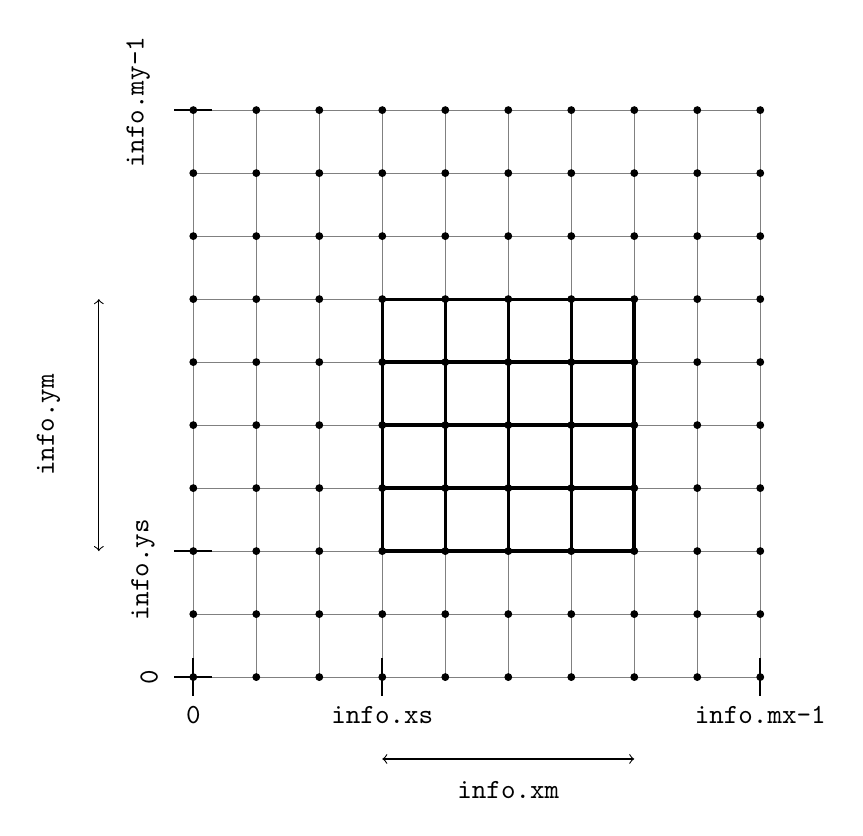
\begin{tikzpicture}[scale=8]
  % global grid, local grid, nodes
  \draw[xstep=0.1,ystep=0.1,gray,very thin] (0.0,0.0) grid (0.9,0.9);
  \draw[xstep=0.1,ystep=0.1,black,very thick] (0.3,0.2) grid (0.7,0.6);
  \foreach \y in {0,...,9}
    \foreach \x in {0,...,9} {
      \filldraw (\x * 0.1,\y * 0.1) circle (0.15pt);
    }
  % ticks on x-axis at 0, xs, mx
  \draw[black,thick] (0,-0.03)   -- (0,+0.03);
  \draw[black,thick] (0.3,-0.03) -- (0.3,+0.03);
  \draw[black,thick] (0.9,-0.03) -- (0.9,+0.03);
  \node at (0,-0.06) {\texttt{0}};
  \node at (0.3,-0.06) {\texttt{info.xs}};
  \node at (0.9,-0.06) {\texttt{info.mx-1}};
  % ticks on y-axis at 0, ys, my
  \draw[black,thick] (-0.03,0)   -- (+0.03,0);
  \draw[black,thick] (-0.03,0.2) -- (+0.03,0.2);
  \draw[black,thick] (-0.03,0.9) -- (+0.03,0.9);
  \node[rotate around={90:(0,0)}] at (-0.07,0) {\texttt{0}};
  \node[rotate around={90:(-0.2,0.2)}] at (-0.08,0.12) {\texttt{info.ys}};
  \node[rotate around={90:(0.0,0.9)}] at (-0.20,0.8) {\texttt{info.my-1}};
  % xm, ym along sides of local patch
  \draw[<->,] (0.3,-0.13) -- (0.7,-0.13);
  \node at (0.5,-0.18) {\texttt{info.xm}};
  \draw[<->,] (-0.15,0.2) -- (-0.15,0.6);
  \node[rotate around={90:(0.3-0.3,0.4)}] at (-0.28,0.35) {\texttt{info.ym}};
\end{tikzpicture}
\caption{A \texttt{DMDALocalInfo} struct describes the indices for a local process' part of a 2D grid, plus the global grid size, using six integers.}
\label{fig:localpartofgrid}
\end{figure}

The index ranges from \texttt{info} are used in the \texttt{for} loops which re-appear every time we do operations on a structured 2D grid:
\begin{code}
for (j=info.ys; j<info.ys+info.ym; j++) {
  for (i=info.xs; i<info.xs+info.xm; i++) {
    DO SOMETHING AT GRID POINT (i,j)
  }
}
\end{code}

Still considering the code in Figure \ref{code:structuredpoisson}, the \pMat object $A$ assembled by \texttt{formdirichletlaplacian()}  has ranges of rows owned by each process, the standard parallel layout \texttt{MATMPIAIJ} of \pMat objects in \PETSc (Chapter \ref{chap:getstarted}).  However, because we work with the locally-owned subgrid using $(i,j)$ indices, we can often forget the actual layout of a \pMat.  We get to just focus on the part of the grid owned by the process instead of worrying about the matrix itself.

In particular, local indices $(i,j)$ can be used when inserting entries into \pMat \texttt{A}, which is really a dynamical data structure for matrix assembly.  Thus in Figure \ref{code:structuredpoisson} we see one use of \texttt{MatSetValuesStencil()} for each locally-owned grid point.  For a generic interior point this command inserts five coefficients into the matrix.  The key data structure is of type \texttt{MatStencil}, an apparently-trivial struct
\begin{code}
typedef struct {
  PetscInt k,j,i,c;
} MatStencil;
\end{code}
In our 2D case, with a single degree of freedom at each node,\sidenote{The Poisson equation \eqref{poissonsquare} is a scalar PDE so the unknown at each grid point is the scalar $U_{i,j}$.  A system of equations like Navier-Stokes would have \texttt{dof}$>1$ when we call \texttt{DMDACreateXd()}, and the ``\texttt{c}'' member of \texttt{MatStencil} would get used.} we only use the \texttt{i} and \texttt{j} members of \texttt{MatStencil}.  From \eqref{poissonsquareFD}, the actual matrix entries are $a_{i,i} = 2\left(h_y/h_x + h_x/h_y\right)$ on the diagonal, and $a_{i,j} = -h_y/h_x$ or $a_{i,j} = -h_x/h_y$ for off-diagonals.  We only insert nonzero off-diagonals in the matrix if the column corresponds to a non-boundary location.


\section{A particular problem, an exact solution}

At this point we need to set up a particular Poisson problem so our example code can solve it.  To do this we again\sidenote{For the code \texttt{tri.c} in Chapter \ref{chap:linearsystem} we did something similar, i.e.~choosing exact solution $\bu$ before computing $\bb=A\bu$ by matrix multiplication.} \emph{choose} an exact solution, taking care that it satisfies homogeneous Dirichlet boundary conditions ($u=0$ along $\partial \mathcal{S}$):
\begin{equation}
u(x,y) = (x^2 - x^4) (y^4 - y^2). \label{exactsolution}
\end{equation}
Then we merely differentiate to get $f = -\grad^2 u$.  Thus \eqref{exactsolution} solves \eqref{poissonsquare} with right side
\begin{equation}
f(x,y) = 2 (1 - 6 x^2) y^2 (1 - y^2) + 2 (1 - 6 y^2) x^2 (1 - x^2).\label{manufacturedf}
\end{equation}
From now on we will refer to $u$ in \eqref{exactsolution} as ``$u_{ex}$'', the exact solution.  This same problem and solution appears in Chapter 4 of \citep{Briggsetal2000}, so these formulas are not original. % page 64

Observe that the truncation error term $O(h^2)$ in equation \eqref{secondderivativeFD} has a coefficient proportional to fourth derivatives \citep{MortonMayers} so our FD method will not be exact on this problem.  That is, $u_{ex}$ has nonzero fourth derivatives.  This is \emph{good}.  We would not want to use the simpler form $u(x,y)=(x-x^2)(y^2-y)$, for example, to test convergence rate of the code because the decay of numerical error with refining grids is not at all generic.

Because we want to reuse this part also,\sidenote{See Chapter \ref{chap:multigrid}.} we put the code that computes formulas \eqref{exactsolution} and \eqref{manufacturedf} in source file \texttt{structuredpoisson.c}.  Figure \ref{code:poissonexactrhs} shows how \eqref{exactsolution} is implemented as \texttt{formExact()} and how \eqref{manufacturedf} is implemented as \texttt{formRHS()}.

\cinputpart{structuredpoisson.c}{c/ch3/}{Methods which assemble the exact solution and the right-hand side of equation \eqref{poissonsquareFD}.}{II}{//FORMEXACTRHS}{//ENDFORMEXACTRHS}{code:poissonexactrhs}

The computations in Figure \ref{code:poissonexactrhs} use only local grid coordinates $(i,j)$, with loops over index ranges as shown in Figure \ref{fig:localpartofgrid}.  \PETSc pointer arithmetic (i.e.~tricks) allows us to index the C arrays we get from \texttt{DMDAVecGetArray()} using $(i,j)$.  When we are done with computing \pVecs we restore the C arrays by calling \texttt{DMDAVecRestoreArray()}, and we explicitly ask for the \pVec objects to be assembled by calling \texttt{VecAssemblyBegin/End()}, just as in Chapter \ref{chap:getstarted}.

\cinputpart{poisson.c}{c/ch3/}{Set up \pDM, \pMat, and \pVec objects, and assemble the linear system.}{I}{//CREATE}{//ENDCREATE}{code:poissoncreate}


\section{Solving the PDE}

The code \texttt{poisson.c} uses our finite difference method \eqref{poissonsquareFD} to solve the Poisson problem with $f$ from \eqref{manufacturedf}.  Figure \ref{code:poissoncreate} shows how \texttt{poisson.c} creates the various objects needed to solve the Poisson problem, namely one \pDM, one \pMat, and three \pVecs.  A \pDM object can compute matrix and vector sizes from the grid dimensions, so we call \texttt{DMCreateMatrix()} and \texttt{DMCreateGlobalVector()} to create \pMat and \pVec objects, respectively.  Then we call methods from \texttt{structuredpoisson.c}, as above, to assemble the matrix and vectors.

\PETSc describes the linear system ``$A\bu=\bb$'' by one \pMat \texttt{A} and two \pVecs (\texttt{u} and \texttt{b}), but, as in Chapter \ref{chap:linearsystem}, the system is solved by a \pKSP Krylov space method solver object.

In Figure \ref{code:poissonsolve} we create the \pKSP object and tell it about \texttt{A} through a call to \texttt{KSPSetOperators()}.  Recall there are two ways \texttt{A} is used, namely as the system matrix and as the ``material'' from which the preconditioner is built; this explains why \texttt{A} appears twice when calling \texttt{KSPSetOperators()}.  We also call \texttt{KSPSetFromOptions()} so that we can change the \pKSP type at runtime (illustrated below).  Solving the system means calling \texttt{KSPSolve()}.  Then we report on the solution by computing the numerical error by the norm $\|u-u_{ex}\|_\infty$.  Finally we wrap up by destroying objects and calling \texttt{PetscFinalize()}.

\cinputpart{poisson.c}{c/ch3/}{Solve using \pKSP, and report on solution.}{II}{//SOLVE}{//ENDSOLVE}{code:poissonsolve}


\section{Runtime controls and viewers}

As a first run do:
\begin{cline}
$ cd c/ch3/
$ make poisson
$ ./poisson -ksp_monitor
\end{cline}
%$
to get output
\begin{cline}
  0 KSP Residual norm 1.020952970432e-01 
  1 KSP Residual norm 2.656923348626e-02 
  2 KSP Residual norm 8.679141000397e-03 
  3 KSP Residual norm 1.557150861763e-03 
  4 KSP Residual norm 2.239919982542e-04 
  5 KSP Residual norm 2.519822315367e-05 
  6 KSP Residual norm 2.152764600588e-06 
  7 KSP Residual norm 2.650467236964e-07 
on 9 x 9 grid:  error |u-uexact|_inf = 0.000763959
\end{cline}
Recall that a default $9\times 9$ grid was chosen in calling \texttt{DMDACreate2d()}.  We see seven iterations of the KSP method, a small final residual norm, and an apparently small numerical error.  It is reasonable to think that we have solved a first PDE problem, but skepticism, and further inspection, is in order.

\begin{marginfigure}
\bigskip
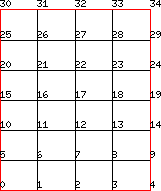
\includegraphics[width=0.8\textwidth]{dmM5N7}
\caption{\PETSc can also graphically show the structured-grid \pDMDA at runtime, here for a single-process run.}
\label{fig:dmM5N7}
\end{marginfigure}

Options \texttt{-da\_grid\_x M -da\_grid\_y N} set the grid at runtime.  Furthermore, we can examine both the grid (i.e.~the \pDM object) and our assembled \pMat graphically at runtime.  If X11 or other windowing is correctly linked in your \PETSc installation then
\begin{cline}
$ ./poisson -da_grid_x 5 -da_grid_y 7 -dm_view draw -draw_pause 5
\end{cline}
%$
gives Figure \ref{fig:dmM5N7}, same as the $M=5$, $N=7$ grid in Figure \ref{fig:unitsquaregrid} with global node ordering by formula \eqref{orderingfd}.  Options
\begin{cline}
$ ./poisson -da_grid_x 5 -da_grid_y 7 -a_mat_view draw -draw_pause 5
\end{cline}
%$
show a graphic similar to Figure \ref{fig:matM5N7}.  This suggests that we have the right kind of matrix structure for the Poisson problem, namely a symmetric sparse matrix with tridiagonal blocks along the diagonal and a banded structure.

\begin{marginfigure}
\bigskip
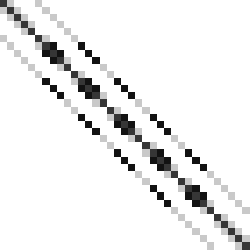
\includegraphics[width=0.95\textwidth]{matM5N7}
\caption{\PETSc can show the matrix structure using X11 windows at runtime.  The actual graphic is in color, but here the two shades of dark gray show positive and negative entries while the light gray shows allocated locations which are zero.}
\label{fig:matM5N7}
\end{marginfigure}

As a specific check on our matrix assembly, this sparse matrix view is easily checked to be identical to the matrix in the linear system on page \pageref{exampleredo}:
\begin{cline}
$ ./poisson -da_grid_x 4 -da_grid_y 3 -a_mat_view
Mat Object:(a_) 1 MPI processes
  type: seqaij
row 0: (0, 1)  (1, 0)  (4, 0) 
row 1: (0, 0)  (1, 1)  (2, 0)  (5, 0) 
row 2: (1, 0)  (2, 1)  (3, 0)  (6, 0) 
row 3: (2, 0)  (3, 1)  (7, 0) 
row 4: (0, 0)  (4, 1)  (5, 0)  (8, 0) 
row 5: (1, 0)  (4, 0)  (5, 4.33333)  (6, -1.5)  (9, 0) 
row 6: (2, 0)  (5, -1.5)  (6, 4.33333)  (7, 0)  (10, 0) 
row 7: (3, 0)  (6, 0)  (7, 1)  (11, 0) 
row 8: (4, 0)  (8, 1)  (9, 0) 
row 9: (5, 0)  (8, 0)  (9, 1)  (10, 0) 
row 10: (6, 0)  (9, 0)  (10, 1)  (11, 0) 
row 11: (7, 0)  (10, 0)  (11, 1) 
on 4 x 3 grid:  error |u-uexact|_inf = 0.0085927
\end{cline}
%$

Finally, a ``movie'' of the \pKSP iterates $\{\bu_k\}$ comes from running
\begin{cline}
$ ./poisson -da_grid_x 100 -da_grid_y 100 -ksp_monitor_solution
\end{cline}
%$
(not shown).  As in Chapter \ref{chap:linearsystem}, a line graph of the (preconditioned) residual norm is from \texttt{-ksp\_monitor\_lg\_residualnorm} (also not shown).  All of the above viewing options can, and probably should, be used on any under-development PDE-solving code on a structured grid.

In fact there are two ways to specify a grid.  One is to specify the grid dimensions directly as above, but the other is to have the \pDM refine the grid by factors of two.  More precisely, the number of \emph{subintervals} is increased by a factor of two.  For example, this option replaces our default grid of 9 by 9 subintervals (i.e.~10 by 10 grid \emph{points}) by 18 subintervals in each direction (i.e.~19 by 19 points):
\begin{cline}
$ ./poisson -da_refine 1
on 19 x 19 grid:  error |u-uexact|_inf = 0.000155374
\end{cline}
%$

In \PETSc the choices of solver and parameters can be made at runtime, once we have adequately-described the problem in terms of \PETSc objects.  We have delayed questions of convergence and efficiency until runtime.  However, now that we have some confidence that we can control our code at runtime, here is what we might want to know:\begin{itemize}
\item is our numerical method correctly implemented? (\emph{convergence})
\item what is going on inside \PETSc? (\emph{exposure})
\item how to get high performance? (\emph{efficiency})
\end{itemize}
In the next three sections we address these in turn, but we only get the most shallow start on efficiency.  Attaining efficiency both requires a better understanding of this goal, and a better appreciation of preconditioning, both of which are addressed in later chapters.


\section{Convergence}

We want to see the numerical errors decrease as we refine the grid.  Such decrease is expected because the finite differences become better approximations of the corresponding derivatives, but we want to \emph{see} it, so we know the code is correct.  Furthermore we want the rate at which the error decreases to match what we expect in theory.

The code \texttt{poisson.c} already generates the max norm error, and we know how to refine the grid by factors of two, so let's generate some  data.  Here is a Bash loop:
\begin{cline}
$ for K in 0 1 2 3 4 5 6; do ./poisson -da_refine $K; done
on 9 x 9 grid:  error |u-uexact|_inf = 0.000763959
on 17 x 17 grid:  error |u-uexact|_inf = 0.000196764
on 33 x 33 grid:  error |u-uexact|_inf = 4.91557e-05
on 65 x 65 grid:  error |u-uexact|_inf = 1.29719e-05
on 129 x 129 grid:  error |u-uexact|_inf = 3.76924e-06
on 257 x 257 grid:  error |u-uexact|_inf = 1.73086e-06
on 513 x 513 grid:  error |u-uexact|_inf = 1.23567e-06
\end{cline}
%$
The data is shown in Figure \ref{fig:poisson-conv} as the squares.  For the four coarsest grids refinement by a factor of two gives a reduction in error by a factor of about four, as expected because our FD method is $O(h^2)$ \citep{MortonMayers}.  Unfortunately the error seems to have stopped falling for the three finer grids, at a numerical error level around $\|u-u_{ex}\|_\infty \approx 10^{-6}$.

\begin{figure}
\bigskip
\includegraphics[width=0.9\textwidth]{poisson-conv}
\caption{To show convergence we refine the \pDM grid by factors of two.  With the default \pKSP relative tolerance the error seems to level out (squares).  With a stronger tolerance for solving the linear system (\texttt{-ksp\_rtol 1.0e-12}) the errors continue to fall (circles) at the expected rate (dotted line).}
\label{fig:poisson-conv}
\end{figure}

Is the reduced apparent rate of convergence a sign of an implementation error?  In fact not, because simply asking for the \pKSP object to solve the linear system more accurately is effective.  On a particular grid we can see the difference using option \texttt{-ksp\_monitor} to watch the residuals and setting a stronger value for the \pKSP relative tolerance for residual norm size (\texttt{-ksp\_rtol}):
\begin{cline}
$ ./poisson -ksp_monitor
  0 KSP Residual norm 1.007660904704e-01 
  1 KSP Residual norm 2.917206076870e-02 
  2 KSP Residual norm 1.153582666339e-02 
... 
  6 KSP Residual norm 6.995040432502e-06 
  7 KSP Residual norm 8.593881990968e-07 
on 10 x 10 grid:  error |u-uexact|_inf = 0.000621778
$ ./poisson -ksp_monitor -ksp_rtol 1.0e-12
  0 KSP Residual norm 1.007660904704e-01 
  1 KSP Residual norm 2.917206076870e-02 
  2 KSP Residual norm 1.153582666339e-02 
...
 13 KSP Residual norm 4.240214646869e-13 
 14 KSP Residual norm 3.105665682224e-14 
on 10 x 10 grid:  error |u-uexact|_inf = 0.000621527
\end{cline}
On this coarse grid the numerical error is nearly the same, but on finer grids the fact that the linear system is solved more exactly will bring the numerical solution closer to the exact one.  However, the \pKSP takes twice as many iterations to achieve the desired residual norm reduction.

In fact, rerunning the Bash loop with the stronger $10^{-12}$ tolerance yields excellent evidence of convergence as shown by the circles in Figure \ref{fig:poisson-conv}.  The linear-fit rate of this logarithmic error data is $O(h^{1.9999})$.  Our implementation is correct.


\section{Exposing \PETSc's options and solvers}

On the other hand, the finer grid calculations above are slow.  How about if we re-run in parallel?  On \WORKSTATION we get:
\begin{cline}
$ timer ./poisson -da_refine 5 -ksp_rtol 1.0e-12
on 289 x 289 grid:  error |u-uexact|_inf = 6.07041e-07
real 31.53
$ time mpiexec -n 4 ./poisson -da_refine 5 -ksp_rtol 1.0e-12
on 289 x 289 grid:  error |u-uexact|_inf = 6.07041e-07
real 12.63
\end{cline}
It is nice to see a speedup, though only by a factor of $31.5/12.6 = 2.5$ on this fixed-size problem, which is disappointing given the putative four-times increase in processing power.

These first performance results may raise more questions than they answer.  In particular,
\renewcommand{\labelenumi}{\roman{enumi})}
\begin{enumerate}
\item are we effectively using \PETSc options at runtime?
\item what is going on inside the \PETSc solver(s)?
\end{enumerate}

Regarding i), even knowing what are the possible runtime options is nontrivial because there are so many.  The first step for finding allowed options is simple: pipe the output from option \texttt{-help} into a pager like \texttt{less}, like this
\begin{cline}
$ ./poisson -help | less
\end{cline}
%$
This gives a view of the options available for those parts of \PETSc which are actually used in \texttt{poisson}.  For instance, the many options for controlling nonlinear solvers and timestepping are \emph{not} included in \texttt{-help} output because we have not used \pSNES or \pTS objects.\sidenote{We get started with \pSNES in Chapter \ref{chap:nonlinear}.}  This \texttt{-help} output also shows the default values for parameters; for example the default for \texttt{-ksp\_rtol} is \texttt{1e-05}, which explains why convergence ``leveled out'' on fine grids in the last section on convergence.

Alternatively, one might want to know what are options for controlling particular objects inside \texttt{poisson}.  For example, we can find the runtime options which control the \pKSP object:
\begin{cline}
$ ./poisson -help | grep ksp_
\end{cline}
%$
If the list is too long, pipe it into the pager:
\begin{cline}
$ ./poisson -help | grep ksp_ | less
\end{cline}
%$

Regarding ii) above, recall that we used \texttt{-dm\_view} to show properties of the \pDM object in \texttt{poisson}, but also we used \texttt{-ksp\_view} in Chapter \ref{chap:linearsystem} to expose the linear solver.  As a reminder here, do
\begin{cline}
$ ./poisson -ksp_view
\end{cline}
%$
We see the serial \pKSP defaults: GMRES plus ILU($0$) as the preconditioner.  And
\begin{cline}
$ mpiexec -n 4 ./poisson -ksp_view
\end{cline}
%$
reminds us that in parallel the defaults are GMRES plus block Jacobi as a preconditioner, but where each diagonal block---there are four here---is preconditioned with ILU($0$).


\section{A first look at efficiency}

On a modestly-fine grid, the \PETSc defaults for \pKSP and \pPC give a certain timing and a certain number of iterations:
\begin{cline}
$ timer ./poisson -da_refine 5 -ksp_converged_reason
Linear solve converged due to CONVERGED_RTOL iterations 506
on 257 x 257 grid:  error |u-uexact|_inf = 1.73086e-06
real 3.77
\end{cline}
%$
That is a lot of iterations, and it is not clear if about 4 seconds is fast or slow.  Without thinking too hard, experimentation should show us what goes faster or slower.  The table below was generated by running
\begin{cline}
$ timer ./poisson -da_refine 5 -ksp_converged_reason -ksp_type KSP -pc_type PC
\end{cline}
%$
and recording the resulting time and iteration count.  The iteration count is worth noting when it can help explain the timing, but at this stage we are identifying the un-defined term ``efficiency'' as just ``execution time.''

\renewcommand{\intime}[1]{\input{timing/poisson/#1}}
\begin{figure}[ht]
\texttt{
\begin{tabular}{llll}
\underline{KSP}\hspace{0.5in} & \underline{PC}\hspace{0.8in} & \underline{\textrm{time (s)}}\hspace{0.3in} & \underline{iterations} \\
gmres      & none        & \intime{gmres.none} \\
           & ilu         & \intime{gmres.ilu} \\
           & ilu + restart=$200$ & \intime{gmres.ilu.restart} \\
cg         & none        & \intime{cg.none} \\
           & jacobi      & \intime{cg.jacobi} \\
           & icc         & \intime{cg.icc} \\
           & icc + rtol=$10^{-14}$ & \intime{cg.icc.tight} \\
minres     & none        & \intime{minres.none} \\
preonly    & cholesky    & \intime{preonly.cholesky}  \\
\end{tabular}
}
\caption{Times and number of \pKSP iterations for serial runs of \texttt{poisson.c} on $257\times 257$ grids.  The assembled matrix is \emph{symmetric}, \emph{diagonally-dominant}, and \emph{positive definite}.  All runs were on \WORKSTATION (see page \pageref{defineworkstation}).} \label{tab:poissontiming}
\end{figure}

From table \ref{tab:poissontiming} we see that for GMRES, having a preconditioner is important and desireable.  That is, ILU($0$) substantially reduces both iteration count and time compared to no preconditioner.  But note that the number of iterations suggests that GMRES went through several restarts, which it does by default every 30 iterations.  For the current problem memory overflow is no issue, so we can try to avoid restart, and in fact that reduces both the iteration count and the time.

FIXME

But wait!  The system matrix $A$ is symmetric and positive definite.  From Chapter \ref{chap:linearsystem} we recall that CG (conjugate gradients) should apply:
\begin{cline}
$ timer ./poisson -da_refine 5 -ksp_converged_reason -ksp_type cg -pc_type none
Linear solve converged due to CONVERGED_RTOL iterations 606
on 257 x 257 grid:  error |u-uexact|_inf = 7.69971e-07
real 1.95
\end{cline}
%$
Thus \emph{un}-preconditioned CG does as well as the above preconditioned forms of GMRES.  This is worth exploring, so let's try two different preconditions which apply to symmetric positive definite matrices; both are mentioned in Chapter \ref{chap:linearsystem}:
\begin{cline}
$ timer ./poisson -da_refine 5 -ksp_converged_reason -ksp_type cg -pc_type jacobi
Linear solve converged due to CONVERGED_RTOL iterations 606
on 257 x 257 grid:  error |u-uexact|_inf = 7.69971e-07
real 2.10
$ timer ./poisson -da_refine 5 -ksp_converged_reason -ksp_type cg -pc_type icc
Linear solve converged due to CONVERGED_RTOL iterations 177
on 257 x 257 grid:  error |u-uexact|_inf = 7.82448e-07
real 1.31
\end{cline}
We see that Jacobi preconditioning seems to make no difference at all,\sidenote{See the exercises.} but that incomplete Cholesky IC($0$) as a preconditioner for CG is the best so far.

We have so far not mentioned the symmetric minimum residual method MINRES \citep{Greenbaum1997}, but of course it is implemented in \PETSc too.  At least in its un-preconditioned form, it seems to do no better that un-preconditioned CG:
\begin{cline}
$ timer ./poisson -da_refine 5 -ksp_converged_reason -ksp_type minres -pc_type none -ksp_rtol 1.0e-14
Linear solve converged due to CONVERGED_RTOL iterations 1044
on 257 x 257 grid:  error |u-uexact|_inf = 7.68279e-07
real 3.56
\end{cline}
%$
Noting that no improvement is theoretically-expected, as CG applies to our positive-definite problem while MINRES only requires symmetry, we will not pursue it further for now.\sidenote{In fact, \citet[][p.~88]{Elmanetal2005} says ``when solving discrete Poisson problems the convergence of MINRES is almost identical to that of CG.''}

While we are at it, however, a ``fair'' comparison to a direct method, in this case Cholesky itself, is in order.  Recall that ``fairness'' means asking for tight convergence tolerance in the iterative method to which we compare:
\begin{cline}
$ timer ./poisson -da_refine 5 -ksp_type preonly -pc_type cholesky
on 257 x 257 grid:  error |u-uexact|_inf = 7.68279e-07
real 27.89
$ timer ./poisson -da_refine 5 -ksp_converged_reason -ksp_type cg -pc_type icc -ksp_rtol 1.0e-14
Linear solve converged due to CONVERGED_RTOL iterations 314
on 257 x 257 grid:  error |u-uexact|_inf = 7.68279e-07
real 2.12
\end{cline}
Because we have several iterative methods that beat it, we conclude that this direct method is not competitive.


\section{Krylov iteration is not enough \dots \emph{good} preconditioning is needed!}

Unfortunately, CG remain seriously flawed, at least from the 21st century point of view.\sidenote{The above timing table might have satisfied in 1975.}  The flaw is that the iteration count grows with refined grids.  In fact, \citet[][p.~76]{Elmanetal2005} summarises the situation this way:
\begin{quote}
for uniformly refined grids, the number of CG iterations required to meet a fixed tolerance will approximately double with each grid refinement
\end{quote}
That is, the 
And this is precisely what we see with another bash loop:
\begin{cline}
$ for NN in 1 2 3 4 5; do
> ./poisson -da_refine $NN -ksp_type cg -pc_type none -ksp_converged_reason; done
Linear solve converged due to CONVERGED_RTOL iterations 36
on 17 x 17 grid:  error |u-uexact|_inf = 0.000196729
Linear solve converged due to CONVERGED_RTOL iterations 73
on 33 x 33 grid:  error |u-uexact|_inf = 4.91819e-05
Linear solve converged due to CONVERGED_RTOL iterations 148
on 65 x 65 grid:  error |u-uexact|_inf = 1.22921e-05
Linear solve converged due to CONVERGED_RTOL iterations 299
on 129 x 129 grid:  error |u-uexact|_inf = 3.07512e-06
Linear solve converged due to CONVERGED_RTOL iterations 606
on 257 x 257 grid:  error |u-uexact|_inf = 7.69971e-07
\end{cline}
Of course, this is un-preconditioned CG.  While it is not surprising that \texttt{-pc\_type jacobi} does no better, such poor scaling unfortunately also applies to our favorite method so far:
\begin{cline}
$ for NN in 1 2 3 4 5; do
> ./poisson -da_refine $NN -ksp_type cg -pc_type icc -ksp_converged_reason; done
Linear solve converged due to CONVERGED_RTOL iterations 12
on 17 x 17 grid:  error |u-uexact|_inf = 0.000196774
Linear solve converged due to CONVERGED_RTOL iterations 23
on 33 x 33 grid:  error |u-uexact|_inf = 4.91531e-05
Linear solve converged due to CONVERGED_RTOL iterations 44
on 65 x 65 grid:  error |u-uexact|_inf = 1.22657e-05
Linear solve converged due to CONVERGED_RTOL iterations 88
on 129 x 129 grid:  error |u-uexact|_inf = 3.0852e-06
Linear solve converged due to CONVERGED_RTOL iterations 177
on 257 x 257 grid:  error |u-uexact|_inf = 7.82448e-07
\end{cline}
%$
We know that IC($0$) gives faster solves and lower iteration counts, but the \emph{scaling} of those iteration counts is the same: doubling with each grid refinement.

FIXME: connect iteration count to condition number i.e.~using result from \citep{Greenbaum1997}

FIXME: \citet[][p.~82]{Elmanetal2005} adds the bad news that 
\begin{quote}
One known result [about CG for the Poisson equation] is that the asymptotic behavior of the condition number using IC(0) preconditioning is unchanged: $\kappa(M^{-1} A) = O(h^{-2})$
\end{quote}

FIXME: but even more bad news: lu beats cg+icc anyway.  this is because lu is applied with nested-dissection () by default, so lu+nd and cholesky+nd are quite good; before dispairing on iteration, however, we are headed toward multigrid
\begin{cline}
$ timer ./poisson -ksp_converged_reason -da_refine 7 -ksp_type cg -pc_type icc -ksp_rtol 1.0e-14
Linear solve converged due to CONVERGED_RTOL iterations 1262
on 1025 x 1025 grid:  error |u-uexact|_inf = 4.80182e-08
real 127.63
$ timer ./poisson -ksp_converged_reason -da_refine 7 -ksp_type preonly -pc_type lu
Linear solve converged due to CONVERGED_ITS iterations 1
on 1025 x 1025 grid:  error |u-uexact|_inf = 4.80182e-08
real 56.45
$ timer ./poisson -ksp_converged_reason -da_refine 7 -ksp_type preonly -pc_type cholesky -pc_factor_mat_ordering_type nd
Linear solve converged due to CONVERGED_ITS iterations 1
on 1025 x 1025 grid:  error |u-uexact|_inf = 4.80182e-08
real 80.00
$ timer ../ch5/fish2 -ksp_converged_reason -da_refine 7 -ksp_type cg -pc_type mg -ksp_rtol 1.0e-14
Linear solve converged due to CONVERGED_RTOL iterations 7
on 1025 x 1025 grid:  error |u-uexact|_inf = 4.80182e-08
real 10.43
\end{cline}
%$

\section{Exercises}

\renewcommand{\labelenumi}{\arabic{chapter}.\arabic{enumi}\quad}
\begin{enumerate}
\item FIXME use \texttt{DMDACreate1d()} to write solver for 1D Poisson
\item FIXME modify \texttt{poisson.c} to do non-homogeneous Dirichlet  
\item Confirm the nearly-identical performance of un-preconditioned and Jacobi-preconditioned CG, by doing
\begin{cline}
$ timer ./poisson -da_refine 5 -ksp_converged_reason -ksp_type cg -pc_type X
\end{cline}
%$
for \texttt{X}=\texttt{none},\texttt{jacobi} in turn.  Explain.
% ANSWER: because all non-boundary condition rows, i.e. all rows with coupling to other equations, which could be split out as A = I \oplus B for B with same condition number as A, have the same diagonal entry of "4" so the only effect of -pc_type jacobi is to scale the spectrum, but the fundamental CG convergence result says CG depends on condition number, i.e. in invariant to scaling of spectrum
\item Add \texttt{-log\_summary} to an un-preconditioned CG run, e.g.
\begin{cline}
$ ./poisson -ksp_converged_reason -ksp_type cg -pc_type none -log_summary
\end{cline}
%$
By looking at the ``Count'' column of ``Event Stage 2: Solve'', and noting the iteration count from the \texttt{-ksp\_converged\_reason} output, confirm that the computational work of one CG iteration consists of two inner products (\texttt{VecTDot}), three vector updates (\texttt{VecAXPY} and \texttt{VecAyPX}), and one matrix-vector product (\texttt{MatMult}).
\end{enumerate}
